\section{Muhammad Tomy (1174031)}
\subsection{Pengertian}
SIG atau Sistem Informasi Geografis dalam bahasa Inggris disebut Geographic Information System disingkat GIS adalah sistem informasi khusus yang mengelola data yang memiliki informasi spasial. SIG juga bias diartikan  dalam arti yang lebih sempit, adalah sistem komputer yang memiliki kemampuan untuk membangun, menyimpan, mengelola dan menampilkan informasi berefrensi geografis, misalnya data yang diidentifikasi menurut lokasinya, dalam sebuah database. Para praktisi juga memasukkan orang yang membangun dan mengoperasikannya dan data sebagai bagian dari sistem ini. Teknologi Sistem Informasi Geografis dapat digunakan untuk investigasi ilmiah, pengelolaan sumber daya, perencanaan pembangunan, kartografi dan perencanaan rute. Misalnya, SIG bisa membantu perencana untuk secara cepat menghitung waktu tanggap darurat saat terjadi bencana alam, atau SIG dapat digunaan untuk mencari lahan basah (wetlands) yang membutuhkan perlindungan dari polusi.


\subsection{Sejarah}
35000 tahun yang lalu, di dinding gua Lascaux, Perancis, para pemburu Cro-Magnon menggambar hewan mangsa mereka, dan juga garis yang dipercaya sebagai rute migrasi hewan-hewan tersebut. Catatan awal ini sejalan dengan dua elemen struktur pada sistem informasi gegrafis modern sekarang ini, arsip grafis yang terhubung ke database atribut.
Pada tahun 1700-an teknik survey modern untuk pemetaan topografis diterapkan, termasuk juga versi awal pemetaan tematis, misalnya untuk keilmuan atau data sensus. Awal abad ke-20 memperlihatkan pengembangan “litografi foto” dimana peta dipisahkan menjadi beberapa lapisan (layer). Perkembangan perangkat keras komputer yang dipacu oleh penelitian senjata nuklir membawa aplikasi pemetaan menjadi multifungsi pada awal tahun 1960-an.
Tahun 1967 merupakan awal pengembangan SIG yang bisa diterapkan di Ottawa, Ontario oleh Departemen Energi, Pertambangan dan Sumber Daya. Dikembangkan oleh Roger Tomlinson, yang kemudian disebut CGIS (Canadian GIS – SIG Kanada), digunakan untuk menyimpan, menganalisis dan mengolah data yang dikumpulkan untuk Inventarisasi Tanah Kanada (CLI – Canadian land Inventory) – sebuah inisiatif untuk mengetahui kemampuan lahan di wilayah pedesaan Kanada dengan memetakaan berbagai informasi pada tanah, pertanian, pariwisata, alam bebas, unggas dan penggunaan tanah pada skala 1:250000. Faktor pemeringkatan klasifikasi juga diterapkan untuk keperluan analisis. CGIS merupakan sistem pertama di dunia dan hasil dari perbaikan aplikasi pemetaan yang memiliki kemampuan timpang susun (overlay), penghitungan, pendijitalan/pemindaian (digitizing/scanning), mendukung sistem koordinat national yang membentang di atas benua Amerika , memasukkan garis sebagai arc yang memiliki topologi dan menyimpan atribut dan informasi lokasional pada berkas terpisah. Pengembangya, seorang geografer bernama Roger Tomlinson kemudian disebut “Bapak SIG”. CGIS bertahan sampai tahun 1970-an dan memakan waktu lama untuk penyempurnaan setelah pengembangan awal, dan tidak bisa bersaing denga aplikasi pemetaan komersil yang dikeluarkan beberapa vendor seperti Intergraph. Perkembangan perangkat keras mikro komputer memacu vendor lain seperti ESRI, CARIS, MapInfo dan berhasil membuat banyak fitur SIG, menggabung pendekatan generasi pertama pada pemisahan informasi spasial dan atributnya, dengan pendekatan generasi kedua pada organisasi data atribut menjadi struktur database. Perkembangan industri pada tahun 1980-an dan 1990-an memacu lagi pertumbuhan SIG pada workstation UNIX dan komputer pribadi. Pada akhir abad ke-20, pertumbuhan yang cepat di berbagai sistem dikonsolidasikan dan distandarisasikan menjadi platform lebih sedikit, dan para pengguna mulai mengekspor menampilkan data SIG lewat internet, yang membutuhkan standar pada format data dan transfer.Indonesia sudah mengadopsi sistem ini sejak Pelita ke-2 ketika LIPI mengundang UNESCO dalam menyusun “Kebijakan dan Program Pembangunan Lima Tahun Tahap Kedua (1974-1979)” dalam pembangunan ilmu pengetahuan, teknologi dan riset.



\subsection{Koordinasi}
Koordinat adalah suatu titik yang didapatkan dari hasil perpotongan dari garis latitude (lintang) dengan garis bujur (longitude) sehingga akan menunjukan lokasi pada suatu daerah. Umumnya koordinat dibedakan menjadi koordinat Geographic dan Universal Transver Mercator (UTM). Pada Koordinat Geogprahic dibedakan menjadi tiga berdasarkan satuannya yaitu :
\begin{itemize}
	\item Degree, Decimal(DD, DDDD) contoh S 4.56734 E 102.67235
	\item Degree,Minute(DD MM,MMMM) contoh S 4 42,5423’ E 105 34,6445’
	\item Degree, Minute, Second(DD MM SS,SS) contoh : S 4 43’ 45,22 E 103 33’ 33,25
\end{itemize}
Pada Bujur/Longitude (X) merupakan garis yang perpindahannya secara vertical dan pada Lintang/Lattitude (Y) merupakan garis yang mempunyai perpindahan secara horizontal.

\subsection{Geospasial}
Data geospasial adalah kumpulan fakta yang berupa informasi tentang ruang kebumian (geospasial) yang menunjukan lokasi atau posisi dari suatu tempat atau objek yang direpresentasikan pada sebuah garis titik koordinat. Data geospasial dibagi menjadi 2 yaitu:
\begin{itemize}
	\item Vektor
	Dalam bentuk data vector bagian objek dibumi ditampilkan sebagai kumpulan titik , garis dan polygon dimana sekumpulan tiitik yang saling terhubung akan membentuk garis dan garis yang saling terhubung antara titik awal dan titik akhir dengan nilai koordinat ynag sama akan membentuk polygon . 

	\item Raster
	Data raster menampilkan permukaan bumi seperti bentuk aslinya atau seperti dalam peta asli yang terlihat jelas dari setiap objek dengan keadaan alamnya. Data raster dibentuk atau menampilkan objek berupa elemen matriks atau grid , data raster digunakan untuk merepresentasikan objek dari data geospasial mengenai batas-batas yang berubah, ketinggian tanah dsb.
\end{itemize}


\subsection{Link}
\href{https://youtu.be/oJ2smVdIph4}{Sistem Informasi Geografis}

\subsection{Plagiarism}
\begin{figure}[H]
	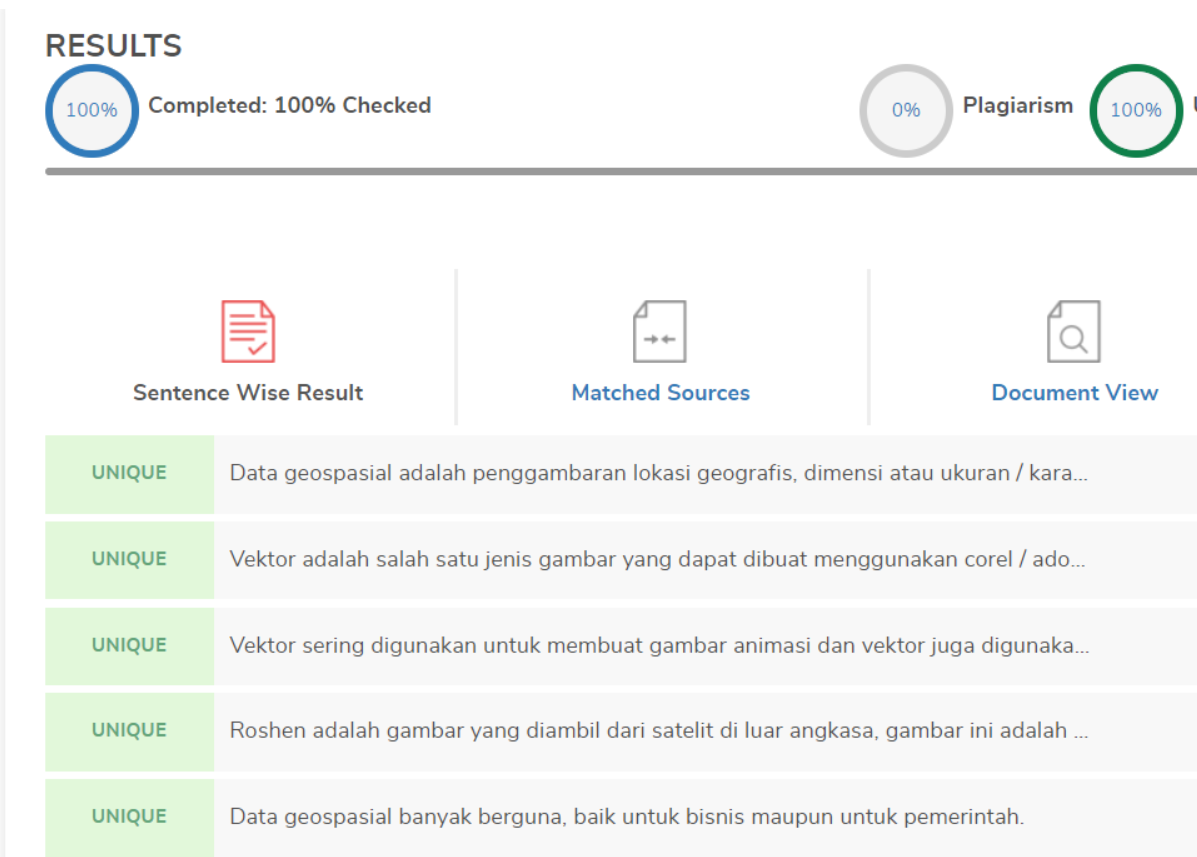
\includegraphics[width=4cm]{figures/1174031/plagiat.png}
	\centering
	\caption{Plagiarism 1174031}
\end{figure}
